% 问题三正文片段；主文件需 amsmath、amssymb、graphicx。
% 与前两问共用 G=(T\cup O,E)、phi、a、pi_k、T_{i,N}、D_{i,N}。
\section{问题三：共享只读 Cache 下的输入自适应调度}

\subsection{建模目标与可执行决策}
问题三沿用场景 B 的 Task 结构：同一核心上的子图合并执行，
跨核依赖通过 DDR 搬运及固定的 $500$ cycle 延迟完成。
新增资源是所有核心共享的只读 FIFO Cache，容量为
$C_{\mathrm{L2}}=1048576\,\mathrm{byte}$，
读带宽为 $\beta_{\mathrm{L2}}=250\,\mathrm{byte/cycle}$。
它与 $\beta=60\,\mathrm{byte/cycle}$ 的 DDR 带宽池相互独立，
不替代容量分别为 $C_{L1}$、$C_{UB}$ 的核内缓存。

本文仍以计算图 $G=(T\cup O,E)$ 为输入，以子图映射 $\phi$、
核心分配 $a$ 和核内子图序列 $\pi_k$ 为决策。
记完整方案为 $\Pi=(\phi,a,(\pi_k)_{k=1}^N)$，其中 $a$ 可由输出序列恢复。
缓存插入、淘汰和指令发射时间均由附件的执行规则决定，
不是可直接提交的变量。因此，缓存协同只能通过合法的切图、
分核和子图顺序间接实现；不向原图添加预热、空操作或等待指令。
总体目标首先是缩短 Makespan，其次是减少额外数据搬运；
命中率用于解释共享输入复用效果，不能单独替代完工时间。

\subsection{从当前输入图构造候选}
对于每个新输入，算法重新建立计算操作 DAG，统计弱连通分量、
拓扑深度、分支与汇合层、各 Pipe 计算周期和张量生产--消费关系。
这些量直接参与构造，不通过用例编号或历史成绩将图归入预设类别。
设分量 $C_j$ 的两管道工作量为
\[
w_j^q=\sum_{o\in C_j:\,p(o)=q}c_o,\qquad q\in\{M,V\}.
\]
按 $\max_q w_j^q$ 降序装箱，先构造完整保留分量的方案。
同一分核映射同时允许两种表达：每核合并为一个子图，
或保留独立分量作为可排序的子图。二者在场景 B 中均合并为一个 Task，
但传入附件的子图顺序不同，可能影响核内确定性排序。
这一区别由当前图的资源模型评价，不能仅凭边界搬运量相同而忽略。

为刻画同核共享输入，另一装箱构造使用增量代价
\begin{equation}
\Delta_{jk}=
\max_{q\in\{M,V\}}\{L_k^q+w_j^q\}
+\frac{\displaystyle\sum_{t\in I_j\setminus I_k}b_t}{\beta},
\label{eq:q3-affinity}
\end{equation}
其中 $L_k^q$ 是核心 $k$ 已分配的管道负载，$I_j$ 为分量的外部输入集合，
$I_k$ 是该核已分配分量的输入并集。式中第二项度量新增输入读取压力，
不预设这些读取必然命中 L2；真实缓存时序在后续轻量事件图中判断。

对于分支与汇合结构，补充独立前缀--汇合尾部、共享前缀--独立输出分支、
分叉--汇合阶段、数据感知深度带和宽度谷切分。
设最大图深为 $h$、总计算工作量为 $W=\sum_{o\in O^{\mathrm c}}c_o$，
分支/汇合层相邻间距集合为 $\mathcal D$。以这些间距的中位数构成
拓扑尺度 $w_{\mathrm{top}}$，取最近整数（半整数取偶）并限于 $[2,32]$；
若间距集合为空，则使用 $\lceil\sqrt h\rceil$ 后作相同截断。
最终尺度为
\begin{equation}
w=\min\left\{h,\,
\max\left[2,w_{\mathrm{top}},
\left\lceil\frac{N\delta_B h}{\max(1,W)}\right\rceil\right]\right\},
\qquad\delta_B=500\,\mathrm{cycle}.
\label{eq:q3-width}
\end{equation}
该式在计算工作量较小时增大切分尺度，以减少同步开销占比。
数据感知深度带只比较 $w$ 与 $2w$ 两种粒度，不连续扫描阈值。
对于相互独立的分量，再允许一次基于共享输入的子图重排；
重排保持数据依赖，不保证或指定某个核心先完成读取。
整个构造集合最多包含十个候选，重复方案在当前调用内去重。

\subsection{双带宽池与 FIFO 的轻量事件模型}
候选必须先通过非 COPY 操作覆盖、子图唯一分配、子图依赖无环
以及依赖与核内顺序合并后无环的检查。
随后依据本图建立一个计算--搬运事件图：
保留操作依赖，在跨核边上计入写回、读入和 $\delta_B$ 释放延迟，
并在各核心的四条 Pipe 上加入串行关系。
计算操作采用原图给定的 $c_o$；传输操作采用原图的 $b_t$。
核内操作的排序采用本模型的拓扑展开，不调用官方核内调度器，
因而这是用于候选比较的近似事件图。

记 $\mathcal Q(t)$ 为时刻 $t$ 已驻留的 FIFO 有序队列。
一个读请求 $j$ 在发射时刻 $t_j$ 按其逻辑张量标识 $\tau_j$ 判定。
记 $\mathcal Q_j^{\mathrm{issue}}$ 为该次发射查询前的缓存状态；
同时间戳下已经处理的完成与插入事件应计入，不能仅取时间的左极限：
\begin{equation}
h_j=\mathbb 1[\tau_j\in\mathcal Q_j^{\mathrm{issue}}],\qquad
p_j=
\begin{cases}
\mathrm{L2},&h_j=1,\\
\mathrm{DDR},&h_j=0.
\end{cases}
\label{eq:q3-hit}
\end{equation}
写回始终进入 DDR 池。初始 $\mathcal Q(0)=\varnothing$；
同时发出的相同输入读取在首次读完成前仍可能全部未命中，
因此重复访问量只能表示复用机会。

对带宽池 $p$，令 $\mathcal A_p(t)$ 为在途搬运集合，
$r_j(t)$ 为请求 $j$ 尚未服务的字节数。在没有加入或完成事件的时段内，
\begin{equation}
r_j(t+\Delta t)=r_j(t)-
\frac{\beta_p}{|\mathcal A_p(t)|}\Delta t,\qquad
\beta_{\mathrm{DDR}}=\beta,\quad
\beta_{\mathrm{L2}}=250\,\mathrm{byte/cycle}.
\label{eq:q3-bandwidth}
\end{equation}
两池分别结算。下一事件取计算完成、搬运完成或跨核释放中的最早时刻；
搬运集合变化后重新计算其完成时间。这一更新使流量守恒，
也避免将计算、搬运和所有依赖边的等待时间简单相加。

COPY\_IN 完成时尝试插入 $\tau_j$。若其已驻留，则保持 FIFO 顺序；
若 $b_{\tau_j}>C_{\mathrm{L2}}$，则不缓存；否则从队首依次淘汰，
直到有空间后插入队尾。按照附件源码，插入检查发生在每次
COPY\_IN 完成时：若一次发射时命中的条目在该读完成前已被淘汰，
完成时仍可能重新插入。这一细节不能用 LRU 或请求发起量累计替代。
这些规则在轻量事件图内确定预计完工时间 $\widehat T_{\mathrm{evt}}$；
由于事件图中的局部排序是近似的，不能把它称为原版评估器的精确复现。

\subsection{核内驻留修正与确定性选择}
共享 L2 不会消除 L1/UB 的容量限制。为识别长期驻留风险，
算法按各核候选顺序扫描张量的产生和使用，分别维护 L1、UB 驻留集合。
申请空间不足时，优先估计换出未来使用最晚、且不是当前操作输入输出的张量；
无持久副本时计一次写回，后续再次使用时计一次读取。
最终得到预计换出换入量 $\widehat B_{\mathrm{spill}}$。
该逐核顺序模型不包含官方 Step 1--3 的完整空间复用补边，
只用于风险校正；若受保护工作集使逐出估计无法继续，
记录超容量风险并作流量修正，不将其作为容量可行性证明。

候选按以下字典序选择：
\begin{equation}
\Pi^\star=
\operatorname*{arg\,min}_{\Pi\in\mathcal C(G,N)}^{\mathrm{lex}}
\left(
\widehat T_{\mathrm{evt}}(\Pi)+
\gamma\frac{\widehat B_{\mathrm{spill}}(\Pi)}{\beta},
\;\widehat B_{\mathrm{copy}}(\Pi)+\widehat B_{\mathrm{spill}}(\Pi)
\right).
\label{eq:q3-objective}
\end{equation}
其中 $\mathcal C(G,N)$ 是当前输入现场生成的合法候选集合，
$\widehat B_{\mathrm{copy}}$ 包含轻量事件图中的 DDR 和 Cache 服务字节。
第一坐标以 cycle 计，第二坐标以 byte 计，仅在第一坐标相同时决定顺序，
体现完工时间优先、搬运量次之的业务目标。
系数 $\gamma$ 表示未显式进入事件图的核内换出对完工时间的修正，
不能理解为硬件带宽的修改。本轮仅对一个全局系数作敏感性比较，
最终取 $\gamma=1$；没有逐例系数或以结果为标签的算法分类器。

\begin{center}
\centering
\fbox{\begin{minipage}{0.94\linewidth}\small
\textbf{算法 3\quad 输入图自适应的 FIFO Cache 协同调度}\par
\vspace{2pt}\hrule\vspace{4pt}
\textbf{输入：}$G=(T\cup O,E)$、核数 $N$、原版固定配置。\par
\textbf{输出：}$\phi$ 与各核序列 $(\pi_1,\ldots,\pi_N)$。\par
\begin{enumerate}
\setlength{\itemsep}{1pt}
\item 从本图提取计算 DAG、弱连通分量、拓扑深度、管道工作量和张量关系。
\item 若 $N=1$，输出整图单核方案，不搜索；否则按式~\eqref{eq:q3-width}
构造至多十个装箱、结构切分与合法重排候选。
\item 逐一检查覆盖与无环性，删除重复方案，并记录拒绝原因。
\item 从空 FIFO 队列启动轻量事件图，以式~\eqref{eq:q3-hit}、
\eqref{eq:q3-bandwidth} 计算 $\widehat T_{\mathrm{evt}}$ 及搬运字节。
\item 按逐核驻留与下一次使用位置估计 $\widehat B_{\mathrm{spill}}$，
按式~\eqref{eq:q3-objective} 选择方案。
\item 仅输出 \texttt{node\_to\_subgraph}、
\texttt{core\_schedules}。诊断量另存文件，不混入提交格式。
\end{enumerate}
\vspace{2pt}\hrule\vspace{2pt}
每次调用均重新执行；不读取历史方案，也不在求解过程中调用官方评估器。
\end{minipage}}
\end{center}
FIFO 时序只参与模型内部比较，正式输出不包含额外操作或指定发射时刻。

\subsection{实验口径与结果}
开发阶段允许利用官方反馈识别机理偏差，但每轮候选均先从原图生成并冻结，
之后才开展官方评估。本轮先验证六项 FIFO/带宽反例和十二组小图--核数组合；
再按规模与连通性预先选取四个开发图，获得二十份冻结候选标签，
比较全局 $\gamma\in\{0,0.25,0.5,1,2,4\}$。另外四图进行冷启动确认。
首轮全量诊断揭示了同核子图表达及切分粒度问题，因此统一增加
同核合并和双倍深度带两个候选，随后重新冻结并生成全部最终方案。
上述历史说明给定图已参与方法开发；最终全量验收检验可复现性和合法性，
不被解释为完全未见分布上的泛化试验。

对图 $i$、核数 $N$ 和同一冻结方案 $\Pi_{i,N}$，分别得到
$T^{0}_{i,N}$（无 L2）与 $T^{L2}_{i,N}$（只读 Cache），定义
\begin{equation}
\begin{aligned}
S^{0}_{i,N}=\frac{T_{i,1}}{T^{0}_{i,N}},\qquad
&S^{L2}_{i,N}=\frac{T_{i,1}}{T^{L2}_{i,N}},\\
R_{i,N}=\frac{T^{0}_{i,N}}{T^{L2}_{i,N}},\qquad
&\overline R_N=\frac1{100}\sum_{i=1}^{100}R_{i,N}.
\end{aligned}
\label{eq:q3-metrics}
\end{equation}
$R_{i,N}$ 隔离了同一调度方案下的缓存收益；与问题二算法的对比
则同时包含调度改变和缓存改变，二者分开报告。
单核不优化，但仍验收其 Cache 配置，故不能预设 $S^{L2}_{i,1}=1$。
命中率按官方的命中字节占可查询总字节比例计算；无 L2 的命中率不适用。
总额外数据搬运量按官方字段记录，它与最终进入 DDR 带宽池的服务字节
不是同一概念，不能通过扣除命中字节擅自修改该指标。

% Q3_RESULTS_BEGIN
最终版本对全部 $100$ 图、$1\sim5$ 核重新生成 $500$ 份方案，
冻结后进行 $1000$ 次开关 L2 的配对官方验收，全部通过。
验收前后核对了 $114$ 份原始附件和全部求解文件的字节哈希；
正式代码包只含输入图求解代码与全局配置，不含历史方案或官方评估器。
表~\ref{tab:q3-results} 中的每项均为 $100$ 个逐图指标的算术平均，
并非总时间之比。
\begin{table}[htbp]\centering
\caption{第三问全量配对结果。无 L2 与 L2 使用同一份冻结方案。}
\label{tab:q3-results}
\begin{tabular}{rrrrr}\hline
$N$ & $\overline S^{0}_N$ & $\overline S^{L2}_N$ & $\overline R_N$ & 字节命中率 (\%)\\\hline
1 & 1.000000 & 1.008622 & 1.008622 & 9.20\\
2 & 2.027353 & 2.032270 & 1.002481 & 16.09\\
3 & 2.826701 & 2.849607 & 1.009093 & 22.13\\
4 & 3.540343 & 3.591397 & 1.017550 & 22.04\\
5 & 4.080391 & 4.193923 & 1.036819 & 26.45\\
\hline\end{tabular}\end{table}
五核平均加速比为 $4.193923$，高于第二问固定算法的 $3.952170$；
总体改善不意味着每一图均占优，故同时保留逐例比较。
在逐图比较中，相对第二问有 68 图改善、
19 图相同、13 图退步。
该比较混合了调度与硬件收益；同方案缓存对照的五核平均比值为
$\overline R_5=1.036819$，二者不可相互替代。
开关缓存的五核对照中，66 图缩短、33 图相同、
1 图变慢。缓存改变了共享带宽服务和指令完成次序，
因此它不构成对所有图的单调加速保证。
\begin{figure}[htbp]\centering
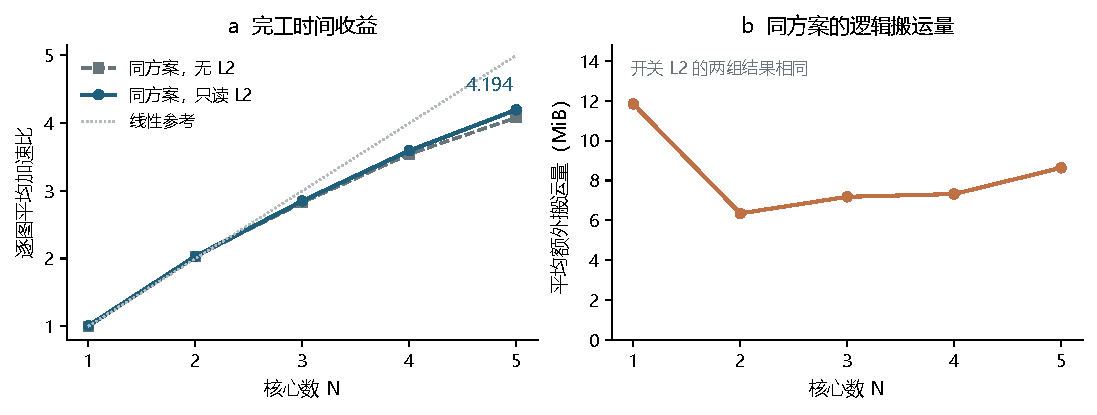
\includegraphics[width=\linewidth]{论文第六章/figures/图6-5_第三问逐核收益与搬运.pdf}
\caption{全量逐核结果。左图比较同方案开启与关闭 L2 的加速比，点为逐图算术均值；
右图为官方额外搬运量。全部配对中该逻辑字节指标相同，因此只绘一条曲线；
这不表示 DDR 实际服务字节相同。单核只采用固定整图方案。}
\label{fig:q3-scaling}\end{figure}
图~\ref{fig:q3-cache} 将字节命中率与完工时间变化分开呈现。
五核散点保留全部用例，命中率高而收益小的点表明，命中率不足以单独预测总体收益。
完整 FIFO 轨迹选取缓存配对收益最大的用例 \texttt{case\_080}，
其选择依据预先写入绘图脚本，不用该用例替代总体结论。
\begin{figure}[htbp]\centering
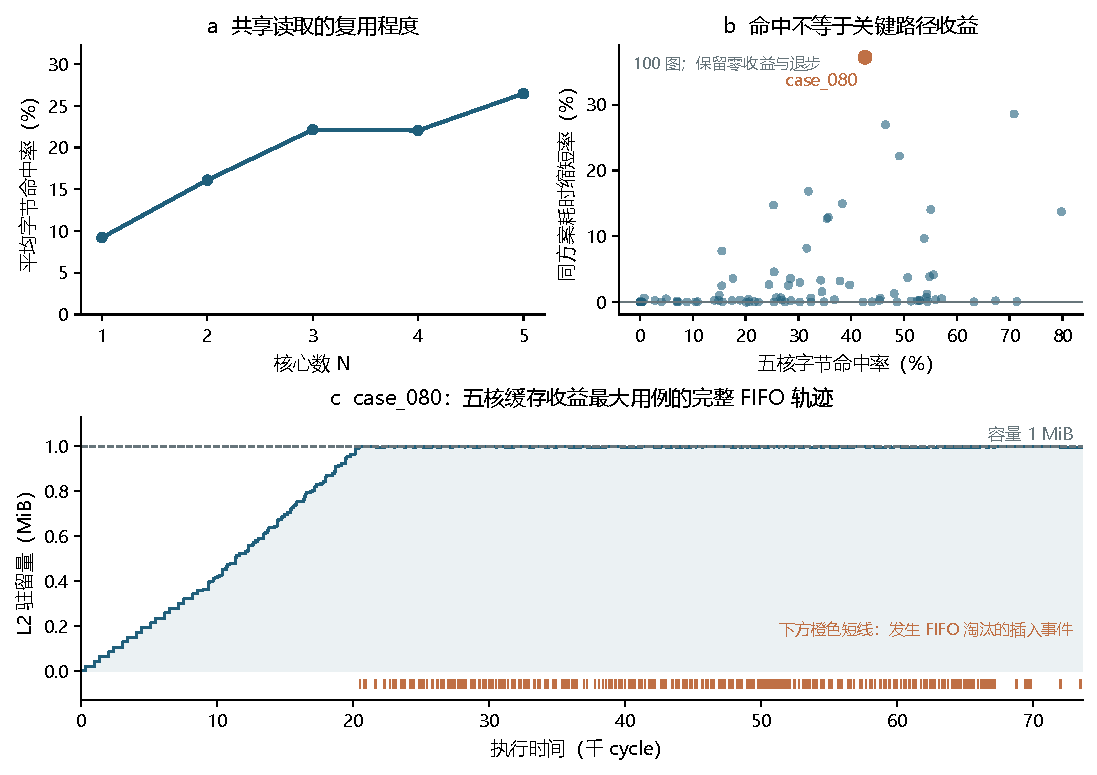
\includegraphics[width=\linewidth]{论文第六章/figures/图6-6_第三问缓存复用与时序.pdf}
\caption{缓存机理与真实时序。a 为各核数的平均字节命中率；b 为全部 $100$ 图的五核配对关系；
c 直接重放缓存收益最大用例的官方插入事件，橙色短线标记伴随淘汰的插入。
事件未下采样，驻留曲线在插入完成时变化；没有人为指定预热或起始时刻。}
\label{fig:q3-cache}\end{figure}
在本机四工作进程并发实验中，$2\sim5$ 核共 $400$ 次独立求解的中位耗时为
$0.600$ s，最长为 $10.916$ s；
去重后候选数中位数为 $7$、最大为 $10$。
这些时间来自进程内计时，包含图读取、构造和模型比较，不含进程启动与官方验收，
也不是专用设备上的串行性能测试。模型以固定规模的构造代替反复试跑官方评估器，
速度和可独立执行性由此获得，代价是保留了局部顺序与换出量近似的误差。
% Q3_RESULTS_END

\subsection{适用边界}
输入自适应来自当前图上的资源计算和有限构造，而非记忆给定测试集的解。
这一实现可以直接接受同格式新图，但可执行接口的独立性不等于分布外性能保证。
轻量事件模型可能因核内排序、空间复用补边或换出重读产生误差；
高命中率也可能对应处于非关键路径的读取，因此不一定带来同幅度的
Makespan 改善。论文的性能结论限于固定硬件配置和已经完成的官方验收。
